\section{Data caching: concept, infrastructure and initiatives}
Simulations of caching layers based on reference WLCG workloads showed a very good ability for latency hiding even when data is read for the first time. The simulations have been conducted using using XCache technology (from the xrootd software framework \cite{xroot}).
Within the root framework \cite{root} it is possible to cache data (reading ahead) while the file starts to be accessed; this is very effective for latencies up to 10 ms when the job configuration parameters are adjusted to the job data accessing patterns (TTreeCache root configuration). For higher latencies the impact starts to be noticeable and CPU inefficiencies grow with increasing latency.\\
In WLCG we have more than 160 sites, all with different roles and scopes e.g. different experiments, local communities, analysis groups, etc. and with a big variety on network topologies and latencies. Sites might have different interests concerning the future of their sites and in particular on their storage services. The new analysis models together with the data lake concept offer more flexibility for sites to re-shape their services according to their needs. An example could be a relatively small Tier-2 currently providing storage and computing to WLCG experiments, needing to maintain a storage system which is of little use to them. If this site is close enough to a the datalake they could consider about accessing data remotely, and if they are on a more distant (in network latency units) place they could interface with data by deploying a stateless storage as a caching layer for latency hiding and eventual file reusability. In Fig. \ref{datalake-sketch} is shown a tentative sketch envisioning a datalake composed by sites and federations holding the bulk of the data regions, and the different types of computing-oriented sites, commercial clouds and HPCs accessing the datalake.\\

\begin{figure}
  \centering
  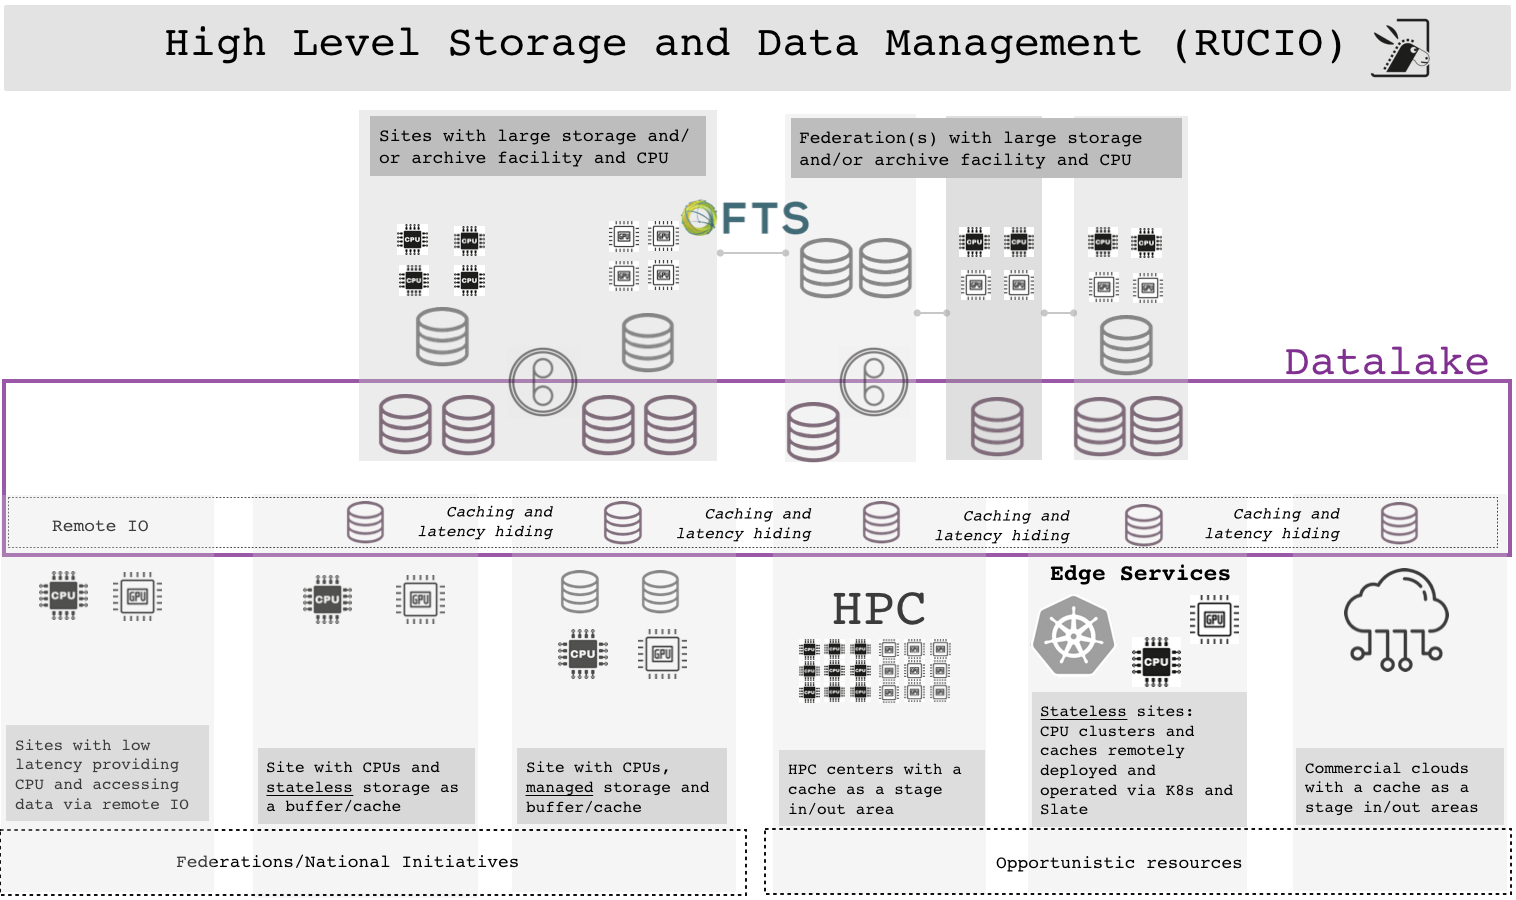
\includegraphics[height=7.8cm]{datalake-sketch-square.png}
  \caption{{\em (center)} Datalake sketch composed by sites and federations holding the bulk of the data regions, and the different types of computing-oriented sites, commercial clouds and HPCs accessing the datalake }
  \label{datalake-sketch}
\end{figure}
The working group has promoted the deployment of several caching models to operate in a region and on a site level. We are investigating three different approaches: a) High performance caching servers in USA to feed a region Southern California (SoCal) and Chicago; and b) caching federation to feed data to regional sites (as in France and Italy); and c) a site caching mechanism as stateless Tier-2 storage (Munich and Birmingham). The results obtained confirm that caching is a promising mechanism to address the analysis challenge and help increasing an efficient usage of the storage and hence able to optimize the overall cost, still meeting the
HL-LHC data storage needs. The caching layer setup at SoCal demonstrates that three sites (Riverside, Caltech and San Diego) can benefit from a common caching layer of 1PB (c.f. with the old model where the site had to deal with 5PB of stateful storage installation), this cache can serve 90\% of the jobs/user request at 1/5th of the cost in hardware and alleviating the site to manage a complex storage service.\\
The initiative in LMU Munich demonstrated that an old disk pool node, with a simple hardware configuration (JBOD) and simple XCache deployment could serve up to 3k concurrent jobs of ATLAS workflows reading data from the neighbour site in Hamburg (DESY) and from a far site in China (IHEP in Beijing). The test concluded that the difference in CPU efficiency when reading from the neighboring site and from the far site is no longer a showstopper taking into account the distance and the latency (Fig. ~\ref{lmu-xcache}).\\

\begin{figure}[h]
  \centering
  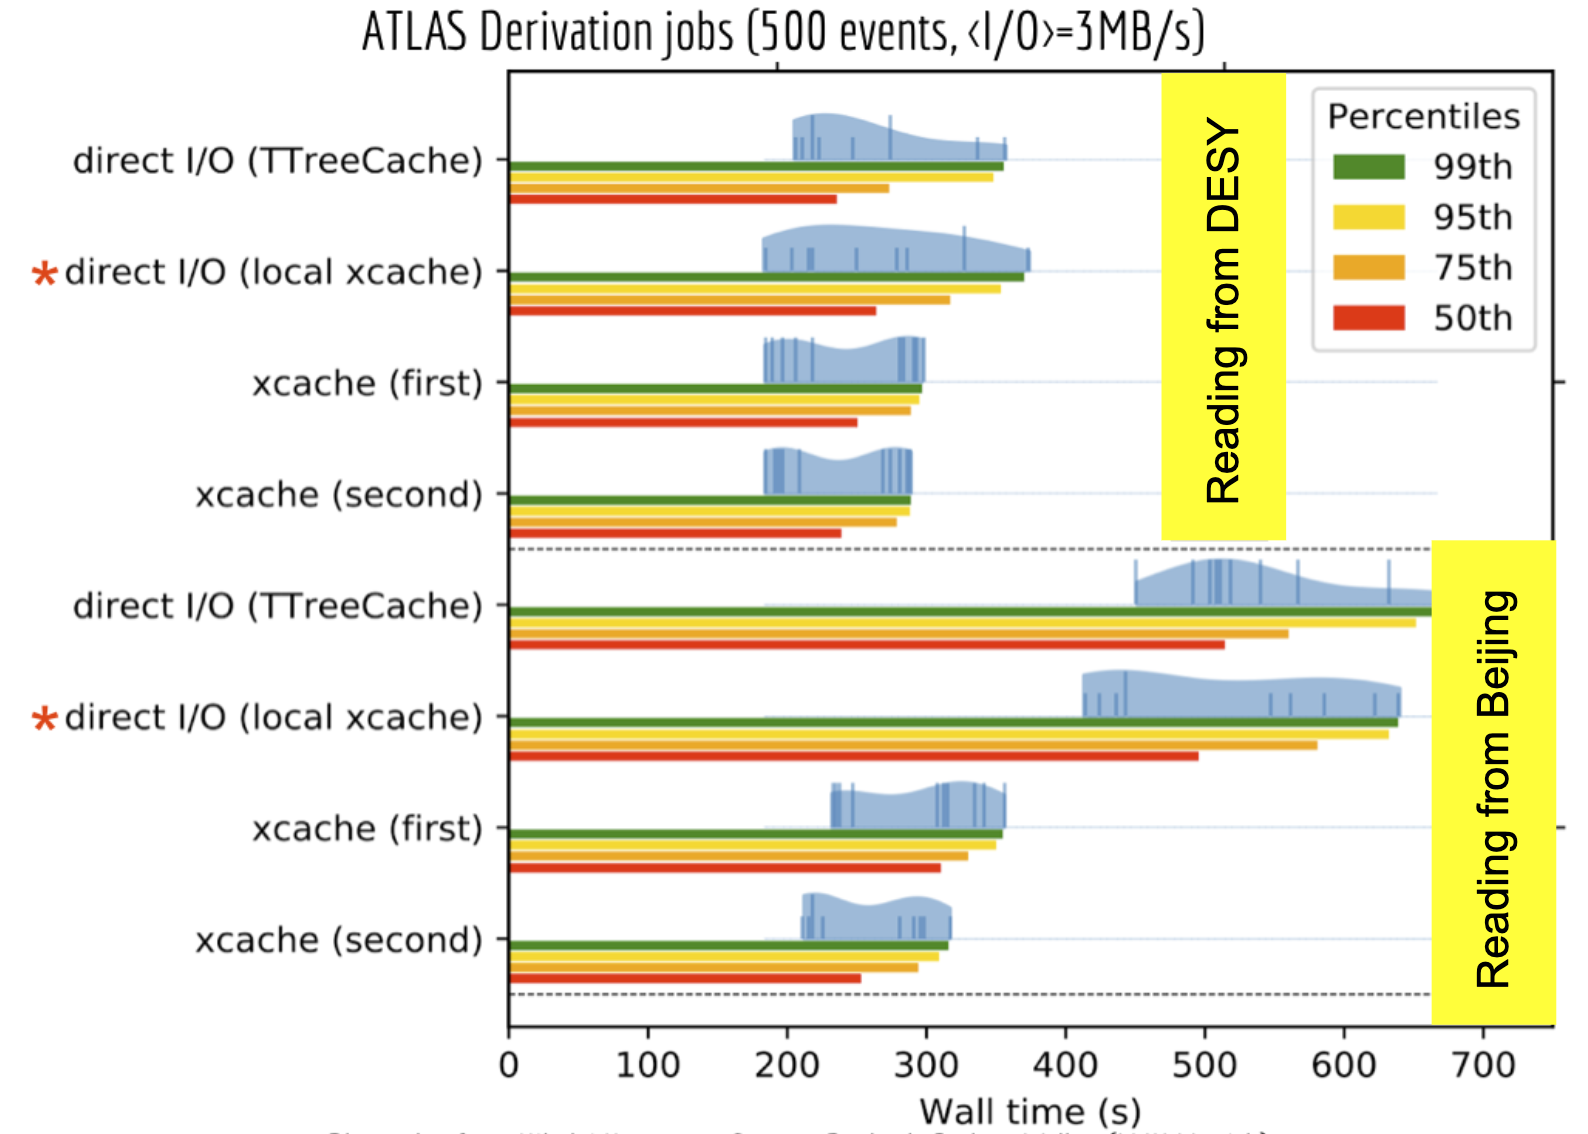
\includegraphics[height=4.5cm]{lmu.png}
  \caption{{\em (center)} XCache running on modest hardware at LMU. Successfully served 3.2k analysis and derivation jobs from ATLAS with and average I/O of 1MB/s and 3MB/s respectively (plot taken from N. Hartman (LMU). Effective latency hiding can be easily achieved for high latency data consumption.}
  \label{lmu-xcache}
\end{figure}




